%% Overleaf			
%% Software Manual and Technical Document Template	
%% 									
%% This provides an example of a software manual created in Overleaf.

\documentclass{../ol-softwaremanual}

% Packages used in this example
\usepackage{graphicx}  % for including images
\usepackage{microtype} % for typographical enhancements
\usepackage{minted}    % for code listings
\usepackage{amsmath}   % for equations and mathematics
\setminted{style=friendly,fontsize=\small}
\renewcommand{\listoflistingscaption}{List of Code Listings}
\usepackage{hyperref}  % for hyperlinks
\usepackage[a4paper,top=4.2cm,bottom=4.2cm,left=3.5cm,right=3.5cm]{geometry} % for setting page size and margins

\usepackage[english, greek]{babel}

\usepackage{subfig}

\usepackage{incgraph,tikz}

\usepackage{filemod}





\usepackage{rotating}


% Custom macros used in this example document
\newcommand{\doclink}[2]{\href{#1}{#2}\footnote{\url{#1}}}
\newcommand{\cs}[1]{\texttt{\textbackslash #1}}

\begin{document}
	
	
	\begin{titlepage}
		
		
		% Frontmatter data; appears on title page
		\title{\en Robustness Diagrams \\}
		\version{0.1}
		\softwarelogo{
\includegraphics[scale=0.4]{../CarBazaar_logo.png}}		
		
	\end{titlepage}
	
	
	\maketitle
	
	\newpage
	
	\center{\textbf{Μέλη Ομάδας}}
	
	\vspace{20pt}
	
	
	
	\begin{table}[htbp!]
		
		\begin{tabular}{llll}
			Μεμελετζόγλου Χαρίλαος & 1069364 & \en st1069364@ceid.upatras.gr & 4o Έτος   \\ 
			\\ Λέκκας Γεώργιος      &      1067430    &   \en st1067430@ceid.upatras.gr & 4o Έτος  \\
			\\ Γιαννουλάκης Ανδρέας        &   1067387       & \en st1067387@ceid.upatras.gr & 4o Έτος           \\
			\\ Κανελλόπουλος Ιωακείμ        &  1070914        &    \en st1070914@ceid.upatras.gr & 4o Έτος        \\ 
		\end{tabular}
	\end{table}
	
	\center{\textbf{Υπεύθυνοι Παρόντος Τεχνικού Κειμένου}}
	
	\vspace{20pt}
	
	\begin{table}[htbp!]
		\begin{tabular}{ll}
			Μεμελετζόγλου Χαρίλαος & \en Editor \\
			\\ Λέκκας Γεώργιος      &   \en  Editor \\
			\\ Γιαννουλάκης Ανδρέας & \en Contributor \\
			\\ Κανελλόπουλος Ιωακείμ & \en Contributor \\ 
		\end{tabular}
	\end{table}
	
	
	\vspace{20pt}
	
	\center{\textbf{Εργαλεία που χρησιμοποιήθηκαν}}
	
	\vspace{20pt}
	\flushleft
	Χρησιμοποιήθηκε το \en \doclink{https://www.overleaf.com/}{Overleaf} \gr και το \en \doclink{https://www.texstudio.org/}{TexStudio} \gr για την συγγραφή του \LaTeX\ κώδικα. \break
	
	Για την δημιουργία του λογότυπου, χρησιμοποιήθηκε το εργαλείο \en \doclink{https://www.adobe.com/express/create/logo}{Adobe Express} . \gr \break
	
	Για την δημιουργία των \en Robustness Diagrams \gr χρησιμοποιήθηκε το \en \doclink{https://www.visual-paradigm.com/}{Visual Paradigm} . \gr \break 
	
	\newpage
	
	\center{\textbf{\en Robustness Diagrams \gr}}
	\flushleft
	
	Οι εναλλακτικές ροές του κάθε \en Use Case \gr φαίνονται στο αντίστοιχο \en Robustness Diagram \gr, με κόκκινες ακμές και αντικείμενα. \break
	
	Για την ευκολότερη αντιστοίχιση ενός \en Use Case \gr στο αντίστοιχο \en Robustness Diagram \gr, παραθέτουμε και το κείμενο της κάθε Περίπτωσης Χρήσης, πρίν το διάγραμμα που προκύπτει. \\
	
	\newpage
	
	\paragraph{\en Use Case 1: \gr Ανάρτηση Αγγελίας Πώλησης Οχήματος}
	\centering
	
	\begin{enumerate}
		
		\item Ο χρήστης επιλέγει \en"\gr Ανάρτηση Αγγελίας Οχήματος\en" \gr στο αρχικού μενού
		\item Το σύστημα εμφανίζει την οθόνη Καταχώρησης Αγγελίας Πώλησης Οχήματος
		\item Ο χρήστης εισάγει την τοποθεσία του, τον τίτλο της αγγελίας, στοιχεία του οχήματος όπως μάρκα, μοντέλο, έτος κυκλοφορίας, χιλιόμετρα, κυβικά, τύπος καυσίμου, χρώμα, αριθμός πινακίδας, κλπ
		\item Το σύστημα ελέγχει πως όντως κυκλοφορεί αντίστοιχο μοντέλο αυτοκινήτου στην αγορά και εμφανίζει στον χρήστη την Οθόνη Ανάρτησης Εγγράφων Πιστοποίησης Κατάστασης Οχήματος
		\item Ο χρήστης ανεβάζει τα απαραίτητα έγγραφα που έχουν προκύψει από τον έλεγχο του οχήματος		
		\item Το σύστημα εμφανίζει στον χρήστη μια εκτίμηση της τιμής του οχήματος, με βάση την κατάστασή του
		\item Ο χρήστης επιλέγει να συνεχίσει με την προτεινόμενη τιμή ή εισάγει δικιά του
		\item Το σύστημα μεταφέρει τον χρήστη στην οθόνη Εισαγωγής Φωτογραφιών και Περιγραφής Οχήματος
		\item Ο χρήστης προσθέτει το κείμενο της περιγραφής και αναρτά τις φωτογραφίες του αυτοκινήτου
		\item Το σύστημα δημιουργεί το \en 3D \gr μοντέλο του οχήματος και εμφανίζει μια προεπισκόπηση της αγγελίας στον χρήστη
		\item Ο χρήστης εγκρίνει την αγγελία
		\item Το σύστημα δημιουργεί την αγγελία και εμφανίζει μήνυμα επιτυχούς ανάρτησης
	\end{enumerate}
	
	\paragraph{Εναλλακτική Ροή 1}
	
	\begin{enumerate}
		\item O χρήστης εισάγει στοιχεία μη-υπαρκτού μοντέλου
		\item Το σύστημα εμφανίζει προειδοποιητικό μήνυμα, επιστρέφει τον χρήστη στην οθόνη \textit{Καταχώρηση Αγγελίας Οχήματος}, προτρέποντάς τον να διορθώσει τα λανθασμένα πεδία
		\item Ο χρήστης προβαίνει στις απαραίτητες διορθώσεις και η Περίπτωση Χρήσης συνεχίζει από το βήμα 4 της βασικής ροής
	\end{enumerate}
	
	\paragraph{Εναλλακτική Ροή 2}
	
	\begin{enumerate}
		\item Ο χρήστης δεν εισάγει περιγραφή ή δεν αναρτά φωτογραφίες του οχήματος
		\item Το σύστημα εμφανίζει προειδοποιητικό μήνυμα, επιστρέφει τον χρήστη στην οθόνη \textit{Εισαγωγή Φωτογραφιών και Περιγραφής Οχήματος}, προτρέποντάς τον, να συμπληρώσει τα αντίστοιχα πεδία
		\item Ο χρήστης εισάγει τις απαραίτητες ελλείπουσες πληροφορίες και η Περίπτωση Χρήσης συνεχίζει από το βήμα 9 της βασικής ροής
	\end{enumerate}
	
	\paragraph{Εναλλακτική Ροή 3}
	
	\begin{enumerate}
		\item Ο χρήστης εισάγει τιμή η οποία είναι σημαντικά μεγαλύτερη από την προτεινόμενη από το σύστημα, τιμή
		\item Το σύστημα εμφανίζει προειδοποιητικό μήνυμα, επιστρέφει τον χρήστη στον οθόνη \textit{Εισαγωγή Τιμής}, προτρέποντάς τον, να εισάγει τιμή που δεν αποκλίνει τόσο από την προτεινόμενη τιμή
		\item Ο χρήστης επανεισάγει τιμή και η Περίπτωση Χρήσης συνεχίζει από το βήμα 8 της βασικής ροής
	\end{enumerate}

	\begin{figure}[htbp!]
		\includegraphics[scale=0.4]{img/rob\_post\_car\_listing.png}
		\caption{\en Robustness Diagram : "\gr Ανάρτηση Αγγελίας Πώλησης Οχήματος\en"\gr}
	\end{figure}
	


	
	\newpage
	
	
	\paragraph{\en Use Case 2: \gr Προγραμματισμός Ελέγχου Οχήματος} 
	
	\begin{enumerate}
		\item Ο χρήστης επιλέγει \en"\gr Έλεγχος Οχήματος\en" \gr στο αρχικό μενού
		\item Το σύστημα εμφανίζει την σελίδα Προγραμματισμού Ελέγχου Οχήματος
		\item Ο χρήστης επιλέγει το πακέτο ελέγχου που επιθυμεί, την ημερομηνία και ώρα διεξαγωγής του ελέγχου και εισάγει την τοποθεσία του
		\item Το σύστημα αφού επιβεβαιώσει την εισαχθείσα τοποθεσία, προτείνει στην χρήστη έναν ελεγκτή, με βάση την τοποθεσία που εισήγαγε
		\item Ο χρήστης αποδέχεται ή όχι τον προτεινόμενο ελεγκτή
		\item Το σύστημα εμφανίζει την οθόνη Εισαγωγή Κωδικού Αγγελίας, στο όχημα της οποίας θα πραγματοποιηθεί ο έλεγχος		
		\item Ο χρήστης εισάγει τον κωδικό της αγγελίας
		\item Το σύστημα ανακτά τα στοιχεία του οχήματος από την αγγελία και εμφανίζει την τελική τιμή του ελέγχου καθώς και την χρονική διάρκειά του
		\item Ο χρήστης επιβεβαιώνει τα στοιχεία
		\item Το σύστημα μεταφέρει τον χρήστη στο μενού πληρωμών. Μετά την επιτυχή πληρωμή, εμφανίζει μήνυμα επιτυχούς κράτησης και αποστέλλει \en email \gr στον χρήστη, με τα στοιχεία του ραντεβού και του ελεγκτή		
	\end{enumerate}
	
	\paragraph{Εναλλακτική Ροή 1}
	
	\begin{enumerate}
		\item Ο χρήστης εισάγει μη-υπαρκτή τοποθεσία
		\item Το σύστημα ενημερώνει τον χρήστη με το κατάλληλο μήνυμα σφάλματος 
		\item Ο χρήστης εισάγει την σωστή τοποθεσία του
		\item Το σύστημα εντοπίζει τον χρήστη και η Περίπτωση Χρήσης προχωρά από το βήμα 4 της βασικής ροής
	\end{enumerate}
	
	\paragraph{Εναλλακτική Ροή 2}
	
	\begin{enumerate}
		\item Ο χρήστης απορρίπτει τον προτεινόμενο από το σύστημα ελεγκτή, προκειμένου να επιλέξει τον ελεγκτή της αρεσκείας του
		\item Το σύστημα εμφανίζει την οθόνη εισαγωγής στοιχείων του ελεγκτή
		\item Ο χρήστης εισάγει τα στοιχεία του ελεγκτή
		\item Το σύστημα ελέγχει πως υπάρχει πράγματι εγγεγραμμένος ο εν λόγω ελεγκτής και αν ναι, η Περίπτωση Χρήσης συνεχίζει από το βήμα 6 της βασικής ροής. Ειδάλλως, εμφανίζει μήνυμα σφάλματος και ο έλεγχος ακυρώνεται	
	\end{enumerate}	


	\begin{figure}[htbp!]
		\includegraphics[scale=0.45]{img/rob\_car\_check.png}
		\caption{\en Robustness Diagram : "\gr Προγραμματισμός Ελέγχου Οχήματος\en"\gr}
	\end{figure}
	
	
	\newpage
	
	\centering
	\paragraph{\en Use Case 12: \gr Ανάρτηση Αγγελίας Πώλησης Ανταλλακτικού \gr}
	
	\begin{enumerate}
		\item Ο χρήστης επιλέγει \en"\gr Ανάρτηση Αγγελίας Ανταλλακτικού \en"\gr στο αρχικό μενού
		\item Το σύστημα εμφανίζει την σελίδα Ανάρτησης Αγγελίας Ανταλλακτικού
		\item Ο χρήστης εισάγει την τοποθεσία του και τον τίτλο της αγγελίας
		\item Το σύστημα εμφανίζει την οθόνη εισαγωγής των στοιχείων του ανταλλακτικού
		\item Ο χρήστης εισάγει στοιχεία του ανταλλακτικού όπως η κατάστασή του (καινούριο ή μεταχειρισμένο), τον τύπο του, τον κωδικό του, την εταιρεία, το μοντέλο και την τιμή του
		\item Το σύστημα ελέγχει πως όντως υπάρχει ανταλλακτικό με τον δοσμένο κωδικό, και στην συνέχεια εμφανίζει την οθόνη Κατηγορίες Ανταλλακτικών, το εντάσσει στην κατάλληλη κατηγορία και προτρέπει τον χρήστη να εισάγει την περιγραφή του ανταλλακτικού αλλά και φωτογραφίες του
		\item Ο χρήστης εισάγει περιγραφή και αναρτά τις απαραίτητες φωτογραφίες
		\item Το σύστημα προτρέπει τον χρήστη να προσφέρει κάποιο ανταλλακτικό χαμηλότερης αξίας ως δώρο μαζί με το κύριο ανταλλακτικό, με σκοπό την ταξινόμηση της αγγελίας του υψηλότερα στα αποτελέσματα αναζήτησης
		\item Ο χρήστης εισάγει τα χαρακτηριστικά και την τιμή του δωρεάν ανταλλακτικού
		\item Το σύστημα εμφανίζει μια προεπισκόπηση της αγγελίας
		\item Ο χρήστης προχωρά στην δημοσίευσή της
	\end{enumerate}
	
	
	\paragraph{Εναλλακτική Ροή 1}
	
	\begin{enumerate}
		\item Ο χρήστης εισάγει κωδικό μη-υπαρκτού ανταλλακτικού
		\item Το σύστημα προειδοποιεί τον χρήστη για το λάθος του
		\item Το σύστημα εμφανίζει μια προειδοποιητική οθόνη και προτρέπει τον χρήστη να εισάγει έγκυρο κωδικό
		\item Ο χρήστης επανεισάγει τον κωδικό και η Περίπτωση Χρήσης προχωρά από το βήμα 4 της βασικής ροής
	\end{enumerate}
	
	\paragraph{Εναλλακτική Ροή 2}
	
	\begin{enumerate}
		\item Ο χρήστης εισάγει ως δωρεάν ανταλλακτικό τιμής της ίδιας τάξης μεγέθους με τον κύριο ανταλλακτικό της αγγελίας
		\item Το σύστημα προειδοποιεί τον χρήστη ενημερώνοντάς τον πως το δεύτερο ανταλλακτικό δεν είναι αρκετά φθηνότερο από το κύριο ανταλλακτικό ώστε να προσφερθεί ως δώρο
		\item Ο χρήστης είτε επιλέγει διαφορετικό ανταλλακτικό ως δώρο είτε προχωρά στην προεπισκόπηση της αγγελίας χωρίς κάποιο δωρεάν ανταλλακτικό και η Περίπτωση Χρήσης προχωρά από το βήμα 9 της βασικής ροής
	\end{enumerate}
	
	\begin{figure}[htbp!]
		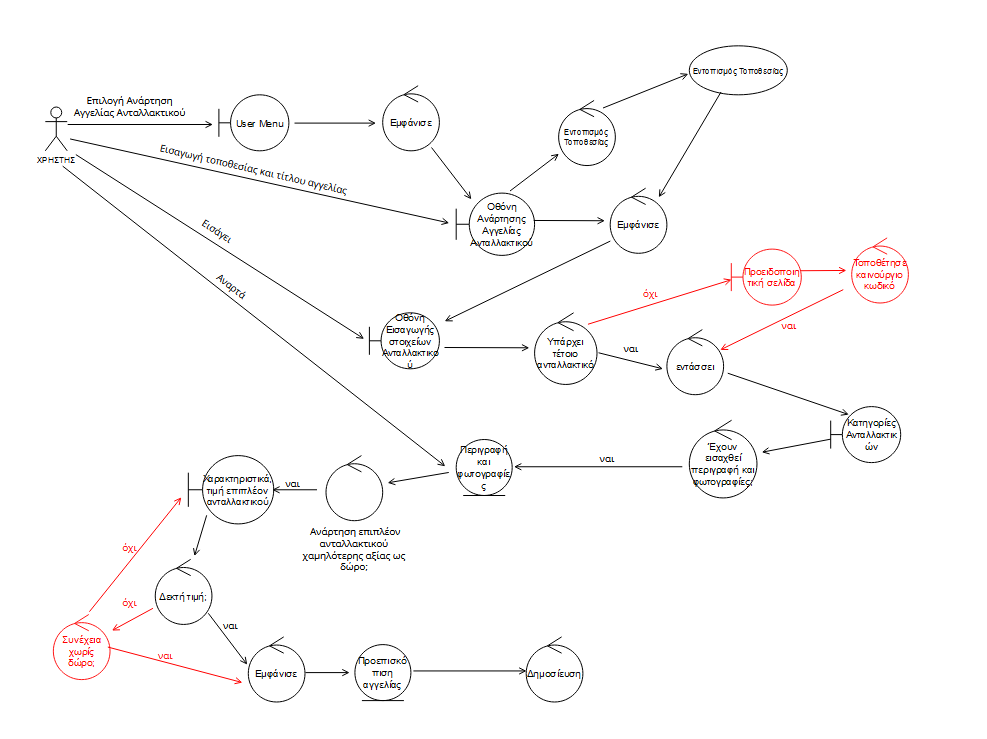
\includegraphics[scale=0.57]{img/rob_spare_part listing.png}
		\caption{\en Robustness Diagram : "\gr Ανάρτηση Αγγελίας Πώλησης Ανταλλακτικού\en"\gr}
	\end{figure}
	
\end{document}



 
